\documentclass[12pt, twoside]{report}  
\usepackage[utf8]{inputenc}
\usepackage[a4paper, width=170mm,top=25mm,bottom=15mm]{geometry}


\usepackage{graphicx}    
\graphicspath{{figs/}} 

\usepackage{float}
\usepackage{caption}
\usepackage{subcaption}  
\usepackage{amsmath}  
\usepackage{amsfonts}
\usepackage{amssymb}   
\usepackage{amsthm}
\usepackage{thmtools}
\usepackage{indentfirst} 
\usepackage{url}
\usepackage{hyperref}
\usepackage{wrapfig}
\usepackage[dvipsnames]{xcolor}
\usepackage{titlesec, color}
\usepackage{ifthen}
\usepackage{etoolbox}



% blue from the logo
\definecolor{mpblue}{HTML}{005E9E}


% Set indentation
\setlength\parindent{0pt}


% Custom title commands
\titleformat{\chapter}
{\color{mpblue}\normalfont\huge\bfseries}
{\color{mpblue}\thechapter.}{1em}{}
\titlespacing*{\chapter}
{0pt}{3.3ex}{3.3ex}

\titleformat{\section}
{\color{mpblue}\normalfont\Large\bfseries}
{\color{mpblue}\thesection.}{1em}{}
\titlespacing*{\section}
{0pt}{3.3ex}{3.3ex}

\titleformat{\subsection}
{\color{mpblue}\normalfont\large\bfseries}
{\color{mpblue}\thesubsection.}{1em}{}
\titlespacing*{\subsection}
{0pt}{3.3ex}{3.3ex}


% Custom headers and footers
\pagestyle{plain}


% maths theorem fields and derivates
\declaretheoremstyle[
  headfont=\color{mpblue}\normalfont\bfseries,
  bodyfont=\color{black}\normalfont\itshape,
]{colored}

\theoremstyle{colored}
\newtheorem{theorem}{Theorem}[section]
\newtheorem{proposition}{Proposition}[section]
\newtheorem{definition}{Definition}[section] 
\newtheorem{lemma}{Lemma}[section] 


% Usefull math operators
\DeclareMathOperator{\rank}{rank}
\DeclareMathOperator{\argmin}{arg\,min}
\DeclareMathOperator{\argmax}{arg\,max}
\DeclareMathOperator{\Tr}{Tr}
\DeclareMathOperator{\sign}{sign}


% Fields for title page
\makeatletter
\newcommand\subtitle[1]{\renewcommand\@subtitle{#1}}
\newcommand\@subtitle{}
\makeatother

\makeatletter
\newcommand\keywords[1]{\renewcommand\@keywords{#1}}
\newcommand\@keywords{}
\makeatother

\makeatletter
\newcommand\logo[1]{\renewcommand\@logo{#1}}
\newcommand\@logo{}
\makeatother

\makeatletter
\newcommand\secondlogo[1]{\renewcommand\@secondlogo{#1}}
\newcommand\@secondlogo{None}
\makeatother

\newcommand\none{None}
\newcommand\includegraphicsifexists[2]{\IfFileExists{#2}{\includegraphics[#1]{#2}}}

% supervisors and roles
\makeatletter
\newcommand\firstsupervisor[1]{\renewcommand\@firstsupervisor{#1}}
\newcommand\@firstsupervisor{None}
\makeatother

\makeatletter
\newcommand\secondsupervisor[1]{\renewcommand\@secondsupervisor{#1}}
\newcommand\@secondsupervisor{None}
\makeatother

\makeatletter
\newcommand\thirdsupervisor[1]{\renewcommand\@thirdsupervisor{#1}}
\newcommand\@thirdsupervisor{None}
\makeatother

\makeatletter
\newcommand\fourthsupervisor[1]{\renewcommand\@fourthsupervisor{#1}}
\newcommand\@fourthsupervisor{None}
\makeatother

\makeatletter
\newcommand\fifthsupervisor[1]{\renewcommand\@fifthsupervisor{#1}}
\newcommand\@fifthsupervisor{None}
\makeatother


\makeatletter
\newcommand\firstsupervisorrole[1]{\renewcommand\@firstsupervisorrole{#1}}
\newcommand\@firstsupervisorrole{}
\makeatother

\makeatletter
\newcommand\secondsupervisorrole[1]{\renewcommand\@secondsupervisorrole{#1}}
\newcommand\@secondsupervisorrole{}
\makeatother

\makeatletter
\newcommand\thirdsupervisorrole[1]{\renewcommand\@thirdsupervisorrole{#1}}
\newcommand\@thirdsupervisorrole{}
\makeatother

\makeatletter
\newcommand\fourthsupervisorrole[1]{\renewcommand\@fourthsupervisorrole{#1}}
\newcommand\@fourthsupervisorrole{}
\makeatother

\makeatletter
\newcommand\fifthsupervisorrole[1]{\renewcommand\@fifthsupervisorrole{#1}}
\newcommand\@fifthsupervisorrole{}
\makeatother


%maketile
\makeatletter
\renewcommand{\maketitle}{
    {\vspace*{2.8cm}}
    {\centering}
    {\LARGE{\textbf{\@title}}}
    
    {\vspace*{0.25cm}}
    {\large {\textbf{\@subtitle}}}
    
    {\vspace{3cm}}
    {\large{\textbf{Author: \@author}}}
    
    {\vspace{2cm}}
    {\large{\textbf{\@date}}}
}
\makeatother



%title
\title{FPGA Wavemeter}
\subtitle{Development of a Field Programmable Gate Array based Wavemeter}
\author{Sourabh Choudhary}
\date{\today}

%keyword
\keywords{ Alexei Ourjoumtsev \\ Sébastien Garcia}

%logo
\logo{figs/logo/ens.png}
\secondlogo{figs/logo/cdf.png}  % optional field

%supervisors - each one of these fields are optional
\firstsupervisor{Alexie Ourjoumtsev}
\firstsupervisorrole{}

\secondsupervisor{2.}
\secondsupervisorrole{Sébastien Garcia}


\DeclareCaptionFormat{custom}
{%
    \centering
    \textbf{#1#2}{#3}
}
\captionsetup{format=custom}



\begin{document}

\pagestyle{empty}


\begin{titlepage}
    \begin{center}
      \makeatletter 
        \begin{figure}[!htb]
          \centering
          
          \ifx\@secondlogo\none
            \begin{minipage}{0.42\textwidth}
            \centering       
            \includegraphics[width=\linewidth]{\@logo}
            \end{minipage}
          \else
            \begin{minipage}{0.42\textwidth}
            \centering       
            \includegraphics[width=\linewidth]{\@logo}
            \end{minipage}
            \hspace{1cm}
            \begin{minipage}{0.42\textwidth}
            \centering       
            \includegraphics[width=\linewidth]{\@secondlogo}
            \end{minipage}
          \fi

        \end{figure}
      \makeatother
      \vspace*{0.25cm}

        \maketitle

        \vspace{2cm}
        \large 
        \textbf{Supervisors}:\\
        \makeatletter
        \textbf{\@keywords}
        \makeatother
        
        \vspace*{\fill}
        \normalsize
        %Conducted under the supervision of: \\
        \vspace{0.5cm}
        \centering
        \makeatletter
        %\begin{tabular}{l c r}
        %\ifx\@firstsupervisor\none  \else \hspace{0.5cm}  \@firstsupervisor       & \hspace{0.25cm}-%\hspace{0.25cm} &  \@firstsupervisorrole \\ \fi 
        %\ifx\@secondsupervisor\none \else \hspace{0.5cm}  \@secondsupervisor      & \hspace{0.25cm}-%\hspace{0.25cm} &  \@secondsupervisorrole \\ \fi
        %\ifx\@thirdsupervisor\none \else \hspace{0.5cm}  \@thirdsupervisor       & \hspace{0.25cm}-%\hspace{0.25cm} &  \@thirdsupervisorrole \\ \fi 
        %\ifx\@fourthsupervisor\none \else \hspace{0.5cm}  \@fourthsupervisor      & \hspace{0.25cm}-%\hspace{0.25cm} &  \@fourthsupervisorrole \\ \fi 
        %\ifx\@fifthsupervisor\none \else \hspace{0.5cm}  \@fifthsupervisor       & \hspace{0.25cm}-%\hspace{0.25cm} &  \@fifthsupervisorrole \\ \fi 
        %\end{tabular}
        \makeatother
        
    \end{center}
\end{titlepage}

\thispagestyle{empty}
\cleardoublepage



\newgeometry{width=140mm,top=40mm,bottom=40mm}

\chapter*{Acknowledgements}
\noindent 

I would like to express my deepest gratitude to my internship supervisors, Dr. Alexei Ourjoumtsev and Dr. Sébastien Garcia, for their guidance, patience, and support during my internship with the Quantum Photonics group of the Young Physics Team at College de France. Their insightful feedback, rigorous attention to detail, and commitment to excellence in research have significantly contributed to my professional growth and learning. I also wish to express my sincere thanks to PhD student Valentin Magro for his help with the lab equipment.
\vspace{1em}

Throughout the course of my internship, their openness and approachability were consistently evident. Whether it was a complex concept that required in-depth explanation or a simple query that needed clarification, they were always willing to invest their time and knowledge. These interactions have been instrumental in enhancing my understanding and deepening my knowledge.
\vspace{1em}

Lastly, I am grateful for the administrative staff who ensure reliable functioning of the establishment and the other interns and visiting students who made the internship experience more lively and enjoyable.This internship has been a milestone in my academic journey, providing me with the necessary tools to face future challenges. Thank you for this incredible opportunity.

\chapter*{Abstract}
\noindent 

This report presents a comprehensive study of a Field Programmable Gate Array (FPGA) based wavemeter designed for high-precision optical wavelength measurements. The wavemeter, which utilizes a Michelson interferometer and custom FPGA circuits, is capable of accurately determining unknown wavelengths by comparing them with a reference laser of known wavelength. The report details the design and operation of the wavemeter, including the setup of optical components, the generation of control signals for the interferometer's translation stage, and the process of wavelength calculation. It also discusses the use of the Edlén Equation for correcting potential errors due to variations in the refractive index of air. The report concludes with a discussion on the practical applications of the wavemeter, particularly in the field of laser wavelength measurement, and provides an outlook on further development to be made for the presented wavemeter.

\newgeometry{width=140mm,top=25mm,bottom=25mm}
\tableofcontents


\newgeometry{width=170mm,top=35mm,bottom=35mm}
\pagestyle{plain}

\chapter{Introduction}\label{chp:intro}

This document presents a comprehensive study of the design, operation, and application of a wavemeter that is in development, a precision instrument used for measuring the wavelength of light. The development of this device was started by a previous intern, LANORE Corentin in 2021. I was given the opportunity to continue building the device. Building on the existing groundwork, while integrating new ideas with the guidance and advice of my supervisors. This process involved understanding the previous work done, identifying areas of improvement, and working on its completion.

\section{Overview}
The wavemeter discussed in this report is based on a Michelson interferometer and utilizes a Field Programmable Gate Array (FPGA) for high-speed data acquisition and processing.

\vspace{1em}
The report begins with an introduction to FPGAs, highlighting their key features and advantages, particularly in the context of high-speed signal processing applications. It also discusses the increasing use of FPGAs in various fields, including quantum technology research, where they are employed for tasks such as Quantum Error Correction and Quantum Key Distribution.

\vspace{1em}
The document then delves into the specifics of the wavemeter, detailing both its hardware and software architecture. The hardware components include lasers, a Michelson interferometer, photodetectors, and the FPGA development board. The software architecture encompasses the Linux environment running on the FPGA board, the custom circuits developed using the Vivado Electronic Design Automation tool, and the web interface for user interaction.

\vspace{1em}
The operation of the wavemeter is explained in detail, starting with the setup of the optical components and the generation of the s-shaped curve for controlling the translation stage of the interferometer. The process of wavelength calculation is then described, including the steps of creating the waves, calculating the wrapped and unwrapped phase, and finally determining the unknown wavelength. The report also discusses the use of the Edlén Equation for correcting potential errors in the wavelength calculation due to variations in the refractive index of air.

\vspace{1em}
This document serves as a comprehensive guide to the design and operation of the wavemeter, providing valuable insights for researchers, engineers, and anyone interested in the field of optical wavelength measurement and FPGA-based signal processing.

\section{Motivation}
The wavemeter is being developed to help measure the wavelenghts of the lasers that are frequently used in the research being done within the group. It simply serves as a way to quickly determine the wavelenght of any laser and ensure that is as per the requirements for the experiments. One of the future goals of the group is do conduct polariton engineering.

\vspace{1em}
Polariton engineering is a field of study that lies at the intersection of quantum physics and materials science. It involves the manipulation and control of polaritons, quasiparticles that are formed from the coupling of photons with an electric or magnetic dipole-carrying excitation. The most commonly studied polaritons are exciton-polaritons, which are hybrid light-matter particles composed of an exciton (an electron-hole pair) and a photon.

\vspace{1em}
Polariton engineering has a wide range of applications, including the development of ultrafast and energy-efficient optoelectronic devices, the study of quantum phenomena at macroscopic scales, and the exploration of new states of matter such as Bose-Einstein condensates and topological insulators \cite{Clark2019}.

\section{Structure}

The structure of this report is organized into several chapters, each focusing on a different aspect of the wavemeter's design, operation, and application. Here is a brief overview of each chapter:

\begin{itemize}
\item \textbf{Chapter 1: Introduction:} This chapter provides an overview of the report and the motivation behind the work. It also outlines the structure of the report.

\item \textbf{Chapter 2: Instrumentation:} This chapter delves into the specifics of the FPGA and the system architecture. It explains the roles of the various hardware components, including lasers, a Michelson interferometer, photodetectors, and the FPGA development board. It also describes the software architecture, which encompasses the Linux environment running on the FPGA board, the custom circuits developed using the Vivado Electronic Design Automation tool, and the web interface for user interaction.

\item \textbf{Chapter 3: Wavemeter Operation:} This chapter explains the operation of the wavemeter in detail. It starts with the setup of the optical components and the generation of the s-shaped curve for controlling the translation stage of the interferometer. It then describes the process of wavelength calculation, including the steps of creating the waves, calculating the wrapped and unwrapped phase, and finally determining the unknown wavelength. The chapter concludes with a discussion on the corrections made using the Edlén Equation.

\item \textbf{Chapter 4: Applications:} This chapter discusses the practical applications of the wavemeter and its limitations in the presented design. 

\item \textbf{Chapter 5: Discussion and conclusion:} This chapter summarizes the key points discussed in the report, highlighting the importance and utility of the wavemeter and FPGA-based signal processing.

\item \textbf{Chapter 6: Outlook:} This chapter gives an outline of the future work that is planned to be done on the wave-meter.

\item \textbf{Appendix:} The appendix contains additional information and data that support the discussions in the main body of the report.
\end{itemize}

Each chapter is designed to provide a comprehensive understanding of the wavemeter, from its basic design principles to its practical operation and application.

\chapter{Instrumentation}
This section first describes the key instrument used in the development of the wavemeter i.e. the Field Programmable Gate Array (FPGA). Then an overview of the entire system, its organisation, the tools used in its development and its intended behaviour is given. 

\section{FPGA}
Integrated circuits can be categorised into two main types, Application Specific Integrated Circuits (ASICs) and Programmable Integrated Circuits (PICs). ASICs are devices that are designed to efficiently perform well defined tasks, for example the CPU and the GPU of a computer. Their behaviour is hard coded and cannot be altered after manufacturing. PICs on the other hand are devices whose functionality can be reconfigured to achieve different desired behaviour. FPGAs are a type of PICs that feature re-configurable components. The development process on an FPGA starts with the use of hardware description language (HDL) like system-verilog to describe the desired functionality of the circuit. This code is passed to an Electronic Design Automation (EDA) tool which is equipped with the knowledge about the components of the FPGA. The EDA tool then describes the configuration for use on the FPGA to achieve the desired functionality. 

\vspace{1em}
\begin{figure}[H]
    \begin{minipage}{0.45\textwidth}
    Figure \ref{fpga-schematic} shows the typical components of an FPGA. The input output blocks shown in green form the interface of between the FPGA and outside electronics. In the case of the FPGA used for the wavemeter the these blocks were connected to a processor, Analog to Digital Signal Converters (ADCs), Digital to Analog Signal Converters (DACs) and other peripherals like memory, expansion connectors etc. The unique component of FPGAs shown in red are the Configurable Logic Blocks (CLBs), these contain generic circuit elements like a collection of hardwired gates, multiplexers, etc. The embedded memory shown in purple is analogous to RAM/ROM on computers, these are inculded within the fabric of the FPGA to enable circuit designs that require fast access to storage. The Digital 
    \end{minipage}%
    \hfill
    \begin{minipage}{0.5\textwidth}
    \centering
    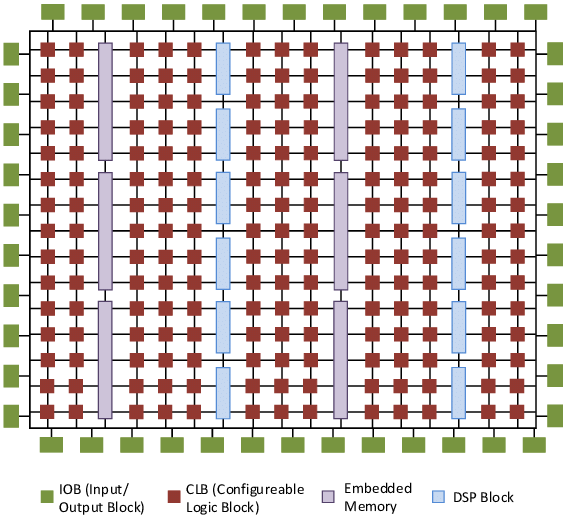
\includegraphics[width=\textwidth]{figs/fpga-schematic.png}
    \caption{Schematic diagram of the components of an FPGA.\cite{fpga-schematic-diag}}
    \label{fpga-schematic}
  \end{minipage}    
\end{figure}

Signal Processing Blocks (DSPs) shown in blue are special purpose blocks that help perform complex mathematical functions at high speeds. Operations like addition, subtraction are simple because the complexity of required circuit scales linearly with the size of the inputs. However, for multiplication the requirement of logic elements scale quadratically with the input size. To address the needs of designs that utilise these operations FPGA are equipped with DSP blocks. These are essential in designs where fast, complex and instantaneous analysis of signals is needed. The black lines in figure \ref{fpga-schematic} that connect all these blocks represent the Programmable Interconnect Points (PIPs), they are the key element used to create the connections between the various blocks as defined by the hardware description code. 

\vspace{1em}
The amount of available elementary blocks on an FPGA determine the complexity of designs that it can be configured to perform. Which is why it is necessary choose an FPGA that has the logic capacity that meets the requirements of the intended design. Other technical elements such as input ouput pins, amount of memory, clock speed should also be considered.  Often, when working with an FPGA it is necessary to define the algorithms to be implemented in a manner such that their circuits can be efficiently designed by the design automation tool. This helps minimise the amount of space used on the FPGA and allows for additional algorithms to be implemented enabling more complex designs. 

\vspace{1em}
These devices have become increasingly popular recently. In the domain of quantum technology and research, they are being used in Quantum Error Correction. Researchers made use of FPGAs' programmable nature to create a system that could monitor parity qubits for quantum states, partially identify errors as they occurred, and correct them on the fly \cite{qec-fpga}. Another study in Quantum Key Distribution utilised FPGAs to handle the high-speed computations required for the sifting, error correction, and privacy amplification processes in their system \cite{Zhang2012}. These studies demonstrate the utility of FPGAs in quantum technology research, serving as examples of how useful they can be in projects where the requirements of the electronic components need to be constantly refined.

\vspace{1em}
For the development of the wavemeter we are studying, a RedPitaya 125-14 FPGA development board was used. The main component of the board is a Xilinx Zynq 7010 system, which features the FPGA and a processing environment that includes an ARM processor, RAM, I/O connectors, etc. RedPitaya, the designer of the development board, added ADCs and DACs and connected them to the FPGA to enable fast (125 MHz) signal processing applications. The development board runs on a custom version of Linux which facilitates interaction between its sub-components and provides a platform for implementing custom circuit designs on the FPGA. These custom circuits are developed using the EDA tool, Vivado. To effectively utilize these devices, one needs to learn a Hardware Description Language like SystemVerilog, become familiar with the development toolchain, understand the architecture of the FPGA, and learn to design algorithms accordingly.

\vspace{1em}

\pagebreak
\section{System Architecture}

This section provides an overview of the the different components of the wavemeter, their configuration and interaction with each other. First we look at the system with a focus on the hardware components which show how the required data is generated and the key specifications of the components involved in the measurement process. Then we look at the system software perspective, which gives an overview of how the generated data is processed.

\subsection{Hardware}

Figure \ref{fig:hw-arch} shows a schematic of how all the key hardware components of the wavemeter are connected. As shown in the figure there are 2 lasers, a reference laser, whose wavelength is known, and another laser with an unknown wavelength. The output of these lasers goes through michelson interferometer and is then connected to two photodetectors (ThorLabs PDA 10A-EC and PDA 10CS-EC) which are connected to the 2 ADCs on the FPGA board. The DAC of the development board connected to an amplifier to make its output range compatible with the piezo stage (PI P-611.1). These components illustrated in yellow blocks are the optical parts of the wavemeter, the experimental setup is explained in detail in section \ref{exp-setup}. The ADCs and DACs are a part of the development board and communicate with the FPGA. For the wavemeter we use a RedPitaya 125-14 FPGA which has 2 ADCs and 2 DACs with a sampling rate of 125 MSa/s. The development board is connected to the local network via an ethernet connection enabling usage with any device on the network. 

\vspace{1em}
\begin{figure}[H]
    \centering
    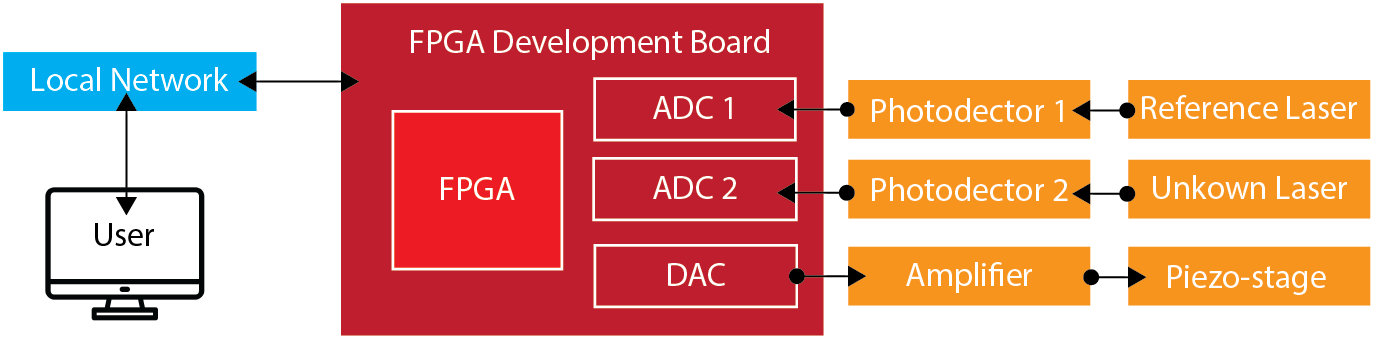
\includegraphics[width=0.9\textwidth]{figs/hw-arch.png}
    \caption{Hardware architecture}
    \label{fig:hw-arch}
\end{figure}

\subsection{Software}

In this section we look at the software architecture of the wavemeter. The development board runs on Linux, it provides the enviorment to interact with the FPGA. The FPGA itself is configured as required by using files generated from the electronic design automation tool, in this case Vivado. Using the hardware description language system verilog, we use the FPGA to process the data from ADCs and DAC. After calculations are done the results are passed to the physical memory of the board. Some C code helps get the data from the memory and it passes it to a python program for further calculations which would be inefficient on the FPGA. The python code also helps in making the data available on a web-interface which makes the process of using the FPGA easy. The front end of the web-interface is desinged using basic HTML and CSS, the backend which gets the required data from the developement board is built using python. This software system can be accessed by any user who is connected to the same network as the development board. 

\begin{figure}[H]
    \centering
    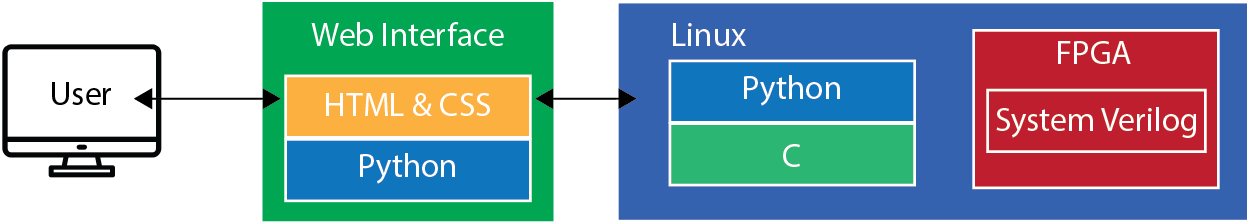
\includegraphics[width=0.8\textwidth]{figs/sw-arch.png}
    \caption{Software architecture}
    \label{fig:sw-arch}
\end{figure}


\chapter{Wavemeter operation}

In this chapter, we examine the operation of the wavemeter. We will explore the key steps involved in determining the unknown wavelength, first we look at the setup of the wavemeter's optical components in section \ref{exp-setup}. Then we look at the curve generation process in section \ref{crv-gen}, which is used to control the translation stage of the wavemeter and start the acquisition of data. Then in section \ref{interfero} we look at how the interference data helps in calculations for the unknown wavelength. In the last section \ref{wavel-extraction} we look at the at how we minimise the error in the calculations.

\section{Apparatus setup}\label{exp-setup}

\begin{figure}[H]
    \centering
    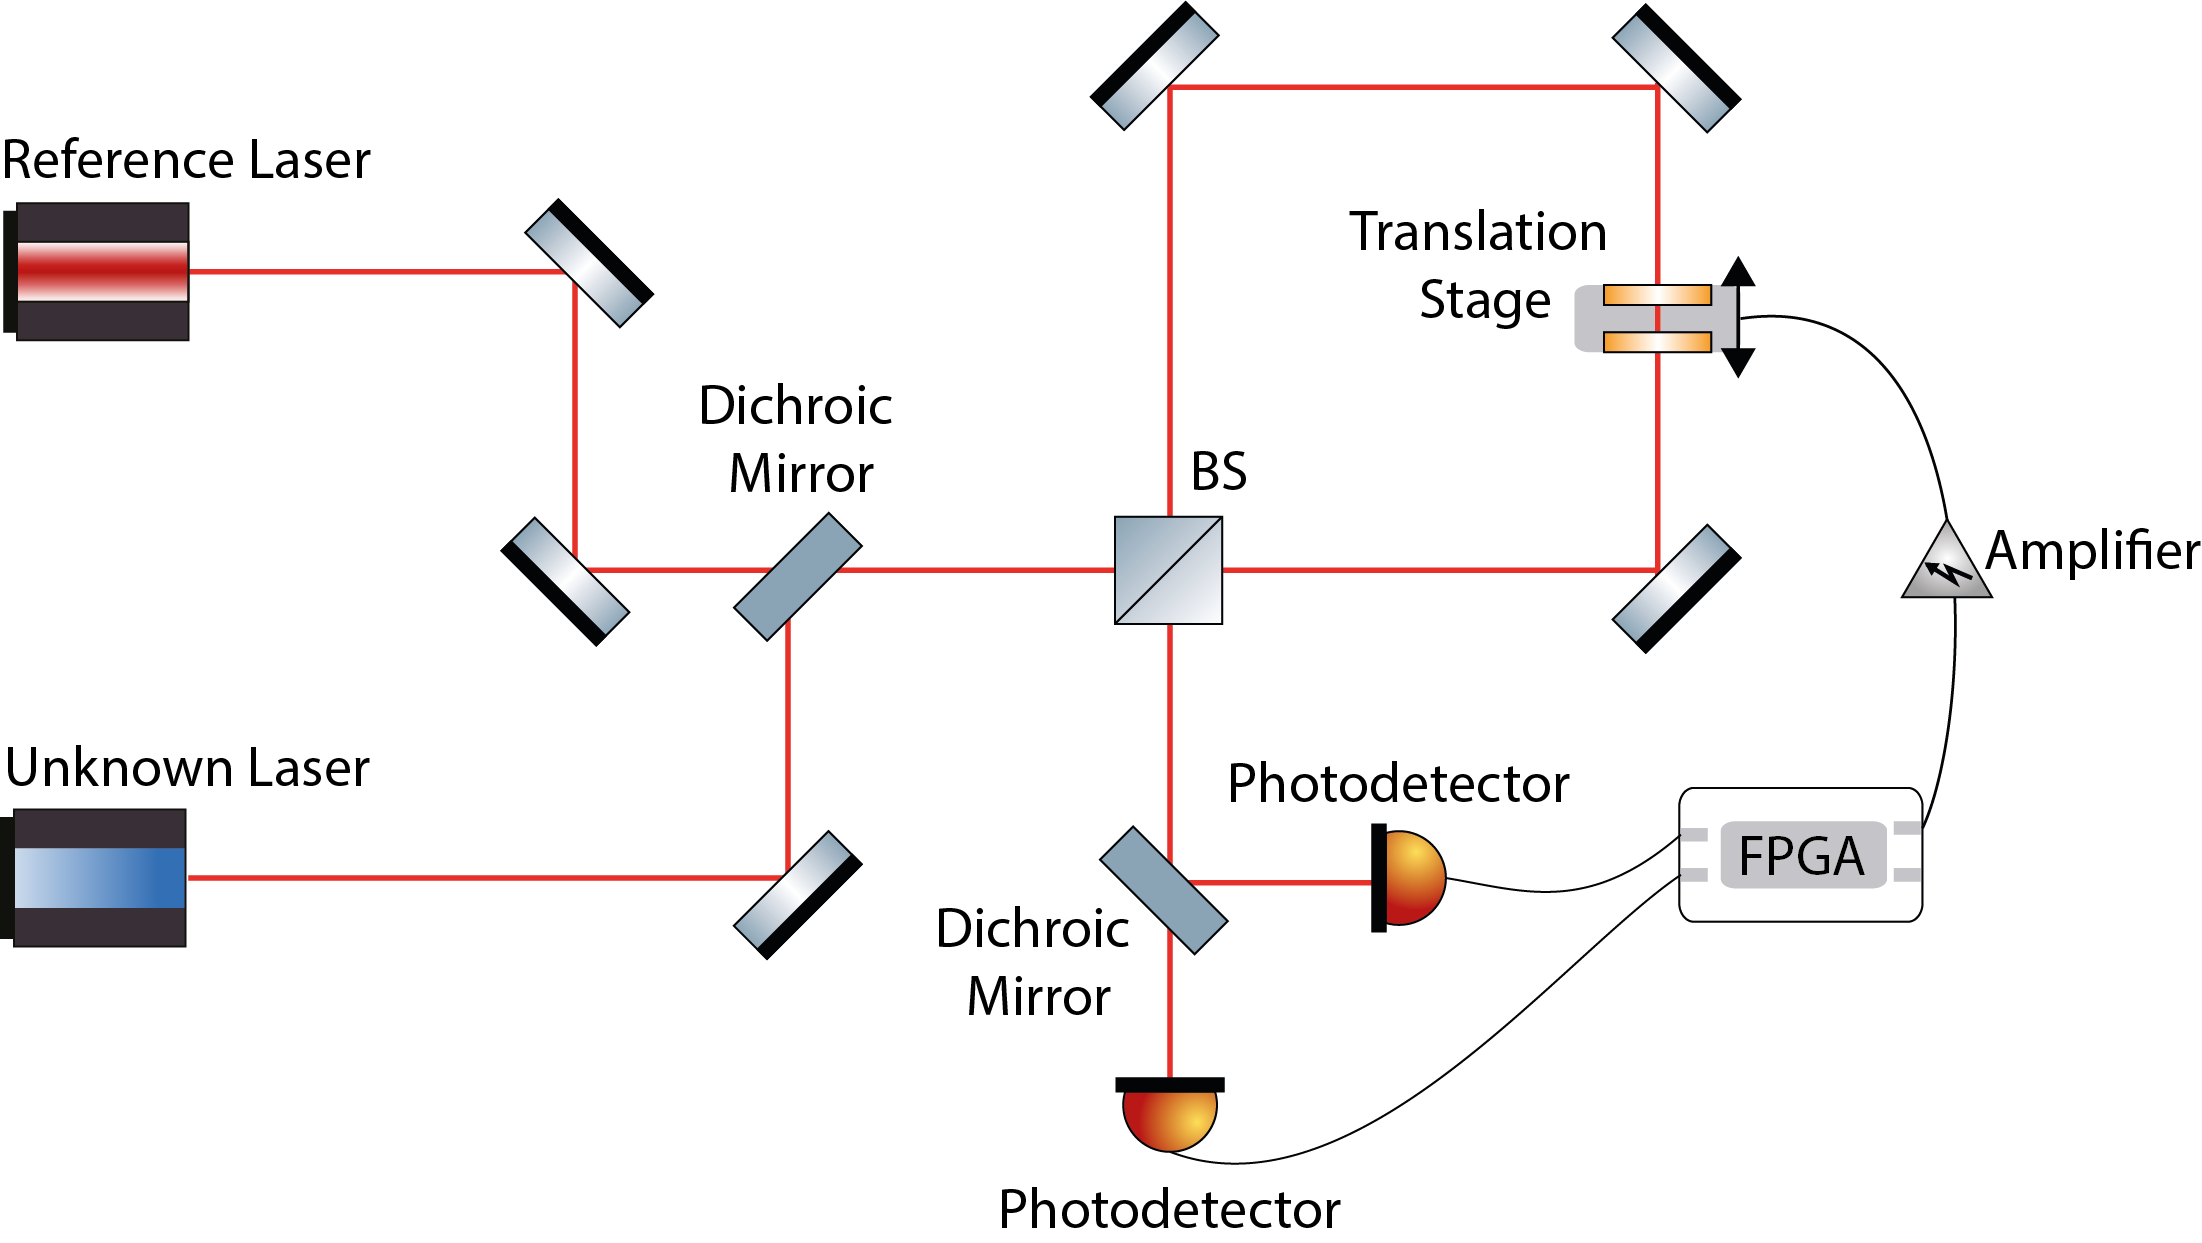
\includegraphics[width=0.8\textwidth]{figs/experimental-setup.png}
    \caption{Experimental Apparatus Setup for the Wavemeter}
    \label{fig:wavemeter-setup}
\end{figure}

Figure \ref{fig:wavemeter-setup} shows how the optical components of the wavemeter are setup. The output beams of the two lasers combine at the dichroic mirror and enter a 50/50 beamsplitter. Then they enter the interferometer which features a translation stage controlled by the DAC of the FPGA. An s-shaped signal is sent via the DAC to move the translation stage by approximately 120 $\mu m$ in 0.067 s, this movement changes the length of the optical path along the arms of the interferometer. After moving the translation stage the two beams exit the interferometer are split again using a dichoric mirror and measured using the photodectors which are connected to the ADCs of the FPGA. The ADCs record and send the data of the interference pattern at a speed of 125 MSa/s, we analyse the phase of both lasers and use it to determine the unknown wavelength.

\section{Curve Generation}\label{crv-gen}

This section describes the technical details of the motion profile used to move the translation stage of the wavemeter. We send an s-shaped curve using the DAC of the FPGA, figure \ref{fig:s-crv} illustrates the trajectory of the motion profile simulated in python and the one generated by the DAC of the FPGA.

\begin{figure}[H]
    \centering
    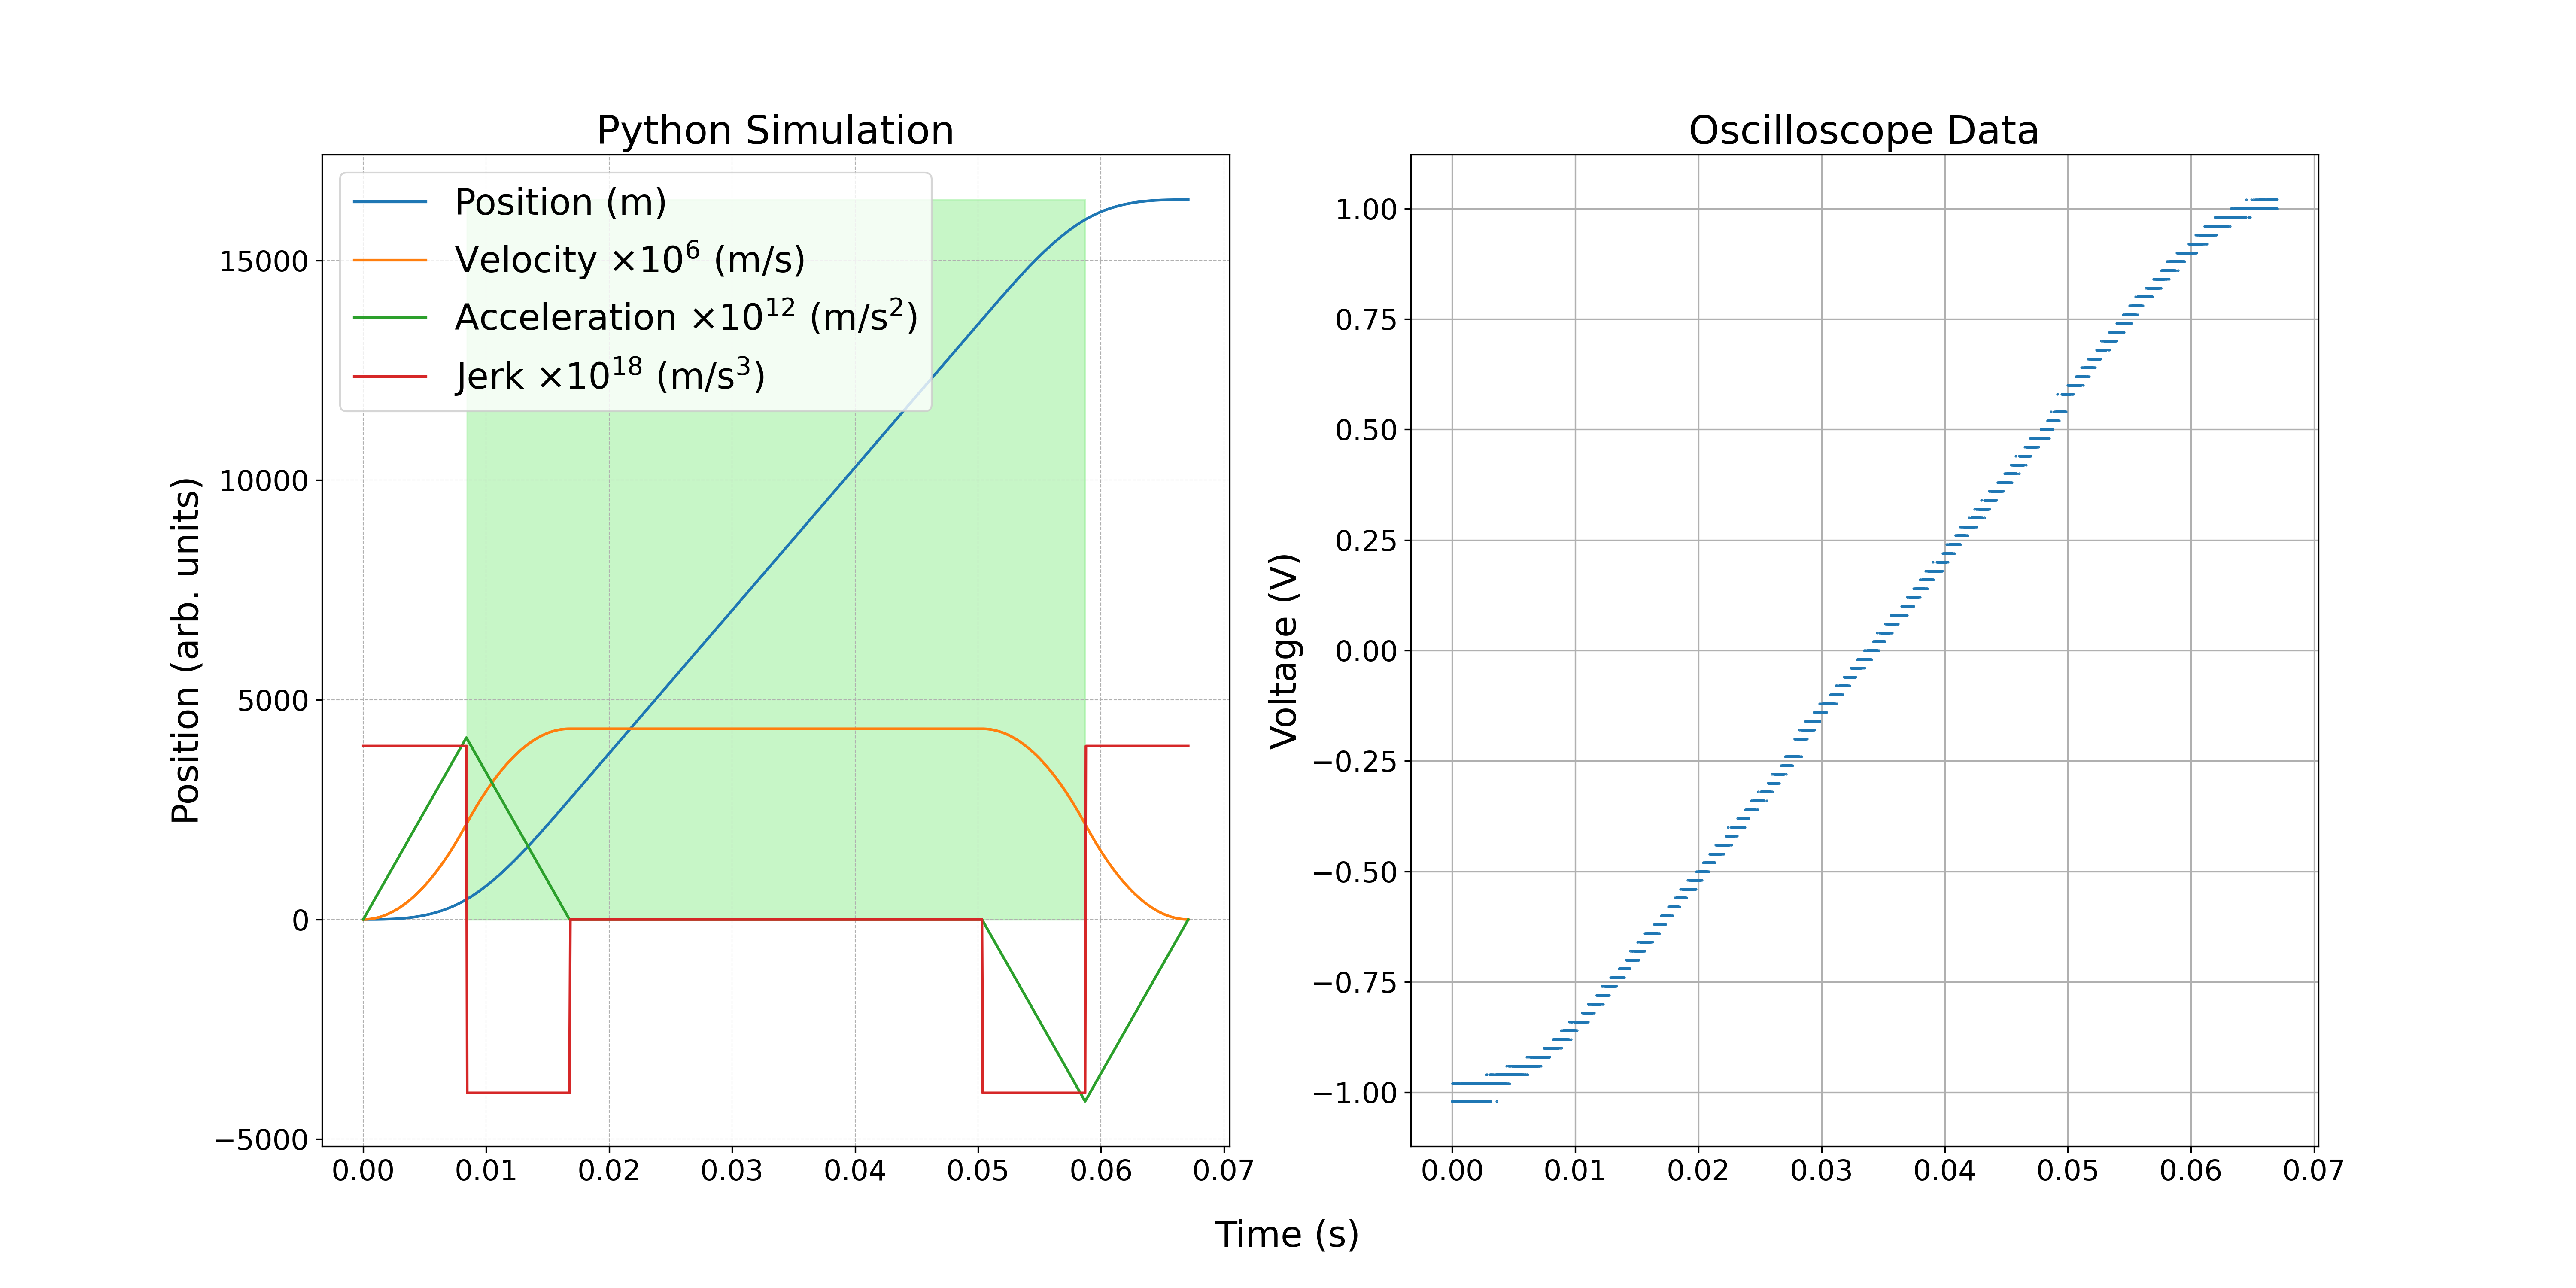
\includegraphics[width=\textwidth]{figs/s-crv.png}
    \caption{{\bf Left :} Simulated trajectory for minimal jerk in python with scaled derivates for visibility. \\ 
    {\bf Right:} Curve captured using a 1 GSa/s oscilloscope for the output of the DAC }
    \label{fig:s-crv}
\end{figure}

From left plot in figure \ref{fig:s-crv} we can see that the s-shaped curve gradually increases acceleration (green line) from zero to its maximum value, and then decreases it back to zero. Similarly, it ramps up deceleration when it's time for the translation stage to stop. This results in a gentler, smoother, and more controlled motion, reducing the mechanical stress and vibrations. The portion shaded in green represents the part of the motion profile where we capture and process the signals from the photodetectors to analyse the phase of the two lasers. The curve shown on the right of figure \ref{fig:s-crv} is generated by the DAC of the FPGA, and shows the voltage of the signal. This signal is amplified from 0 V to 105 V to drive the translation stage. 

\vspace{1em}
The simulation was designed with respect to the clock frequency of the FPGA (125 MHz). As highlghted in green we aim to capture the interference data over a total scan length of 5 ms. To minimise the vibrations induced by the translation stage, we need to apply the jerk profile illustrated in red. The total duration of the the s-signal is 0.0671s, and we determined the constant jerk by taking the triple integral of the position to be :

\begin{equation}
    j = 3.9474 \cdot 10^{-16} \times \frac{m}{s^3}
\end{equation}

As illustrated in figure \ref{fig:s-crv} the jerk profile has this constant positive jerk for the initial part of the curve, and then the same as a constant negative jerk. Followed by a period of 0 jerk, then near the end of the curve it again has the same constant negative jerk, ending with the constant positive jerk. 

\vspace{1em}
Since it is not possible to work with such large precise numbers on the FPGA, the calculations had to made programmable.This was done by keeping multiplication operations within the limits of the DSPs of the FPGA (18 bits $\times$ 18 bits), and wherever making larger multiplication operations and division operations as multiplication by powers of 2 so that they can be programmed as 'bit-shifts' which can be computed efficiently. 

\vspace{1em}
The following equations show how the position is calculated along each step of the jerk profile, for the first part with the constant positive jerk we use

\begin{equation}
y_{p o s}=j \cdot 2^{3 \cdot\left(n_1+n_2\right)} \cdot\left(\left(\frac{\left(\frac{t}{2^{n_1}} \cdot \frac{t}{2^{n_1}}\right)}{2^{n_2}} \cdot \frac{t}{2^{n_1}}\right) \cdot \frac{1}{2^{n_2}} \right) \cdot \frac{1}{2^{n_2}}
\label{eq:pos-j1}
\end{equation}

\vspace{0.5em}
where $y_{pos}$ is the position, $n_1 = 6$ and $n_2 = 17$ are constant parameters that reduce the multiplication and division operations to bit-shifts. We choose these values for $n_1$ and $n_2$ because they reduce bit width of the multiplicands under 18 bits wide, while maintating the enough precision to generate a smooth curve. This ensure that the required calculations are within the limits of the DSPs of FPGA and that they can be done quickly within the required time limit. The variable $t$ is the counter that increments at each clock cycle of the FPGA, the entire curve is generated with this counter going from 0 to $2^{23}$. Equation \ref{eq:pos-j1} is used while the counter goes from 0 to $2^{20}$.

\vspace{1em}
For the initial part with the negative jerk where the counter $t$ goes from $2^{20}$ to $2^{21}$ we use,

\begin{equation}
y_{neg}=y_{n g t}-y_{p o s}-\left(\frac{6 \cdot j \cdot 2^{3\left(n_1+n_2\right)}}{2^{n_2}} \cdot \frac{t}{2^{2 \cdot n_1}}\right)+910
\label{eq:3}
\end{equation}

where, 

\begin{equation}
y_{ngt}=\left(\frac{6 \cdot j \cdot 2^{3\left(n_1+n_2\right)}}{2^3} \cdot \frac{\left(\frac{t}{2^{n_1}} \cdot \frac{t}{2^{n_1}}\right)}{2^{n_2}}\cdot \frac{1}{2^{n_2}}\right)
\label{eq:2}
\end{equation}

\vspace{0.5em}
for the portion with constant velocity and 0 jerk, that begins at $t = 2^{21}$ to $t = 6 \times 2^{20}$ we use the following equation.

\begin{equation}
y_{c s t v}=\frac{6 \cdot j \cdot 2^{3\left(n_1+n_2\right)}}{2^{n_2}} \cdot \frac{t -2^{20}}{2^{2 \cdot n_1}}
\label{eq:5}
\end{equation}

\vspace{1em}
Towards the end of the s-curve, for the portion of negative jerk, where $t= 6 \times 2^{20}$ to $t = 7 \times 2^{20}$ we use,

\begin{equation}
y_{n e g 2} = 2^{14} - \left( \frac{j \cdot 2^{3 \cdot\left(n_1+n_2\right)}}{2^{n_2}} \right) \left( \frac{1}{2^{n_2}} \right) \left( \left(\frac{\left(\frac{2^{23}-t}{2^{n_1}} \cdot \frac{2^{23}-t}{2^{n_1}}\right)}{2^{n_2}} \cdot \frac{2^{23}-t}{2^{n_1}}\right) \cdot \frac{1}{2^{n_2}} \right)
\label{eq:6}
\end{equation}

\vspace{0.5em}
here, we exploit the symmetry in the s-curve by subtracting the $t$-terms from $2^{23}$ and the result by $2^{14}$ which is the maximum position because the DAC has a max bitwidth of 14 bits. 

\vspace{1em}
Similarly, for the last part with the positive jerk, where $ t = 7 \times 2^{20}$ to $t = 2^{23}$ we use, 

\begin{equation}
y_{p o s}= 2^{14} - j \cdot 2^{3 \cdot\left(n_1+n_2\right)} \cdot\left(\left(\frac{\left(\frac{2^{23}-t}{2^{n_1}} \cdot \frac{2^{23}-t}{2^{n_1}}\right)}{2^{n_2}} \cdot \frac{2^{23}-t}{2^{n_1}}\right) \cdot \frac{1}{2^{n_2}} \right) \cdot \frac{1}{2^{n_2}}
\label{eq:pos-j1-s}
\end{equation}

\vspace{0.5em}
This completes the s-curve. This curve can be generated simply by a clicking a switch and has been programmed to synchronously start the interference acquisition at the point where constant velocity begins.

\section{Wavelength calculation}\label{interfero}

This section gives details about how the unknown wavelength is calculated from the input data of the ADCs. We look at the step-by-step calculations used to determine the unknown wavelength. The results of each step is visualised using oscilloscope data. Since, the wavemeter is still under development, we use a frequency generator as the input to the ADCs. It serves as a placeholder for the input from the photodetectors.

\begin{enumerate}
\item \textbf{Creating the waves:} Using the frequency generator, two sine waves of 100 kHz and 200 kHz with an amplitude of 2V were generated as shows in figure \ref{fig:waves-in}. Here, the 100 kHz wave simulates the reference laser, with the known wavelength. The 200 kHz signal simulates the laser with unknown wavelength. We will compare the results with calculations from the FPGA to verify that the implementation works reliably. 

\begin{figure}[H]
    \centering
    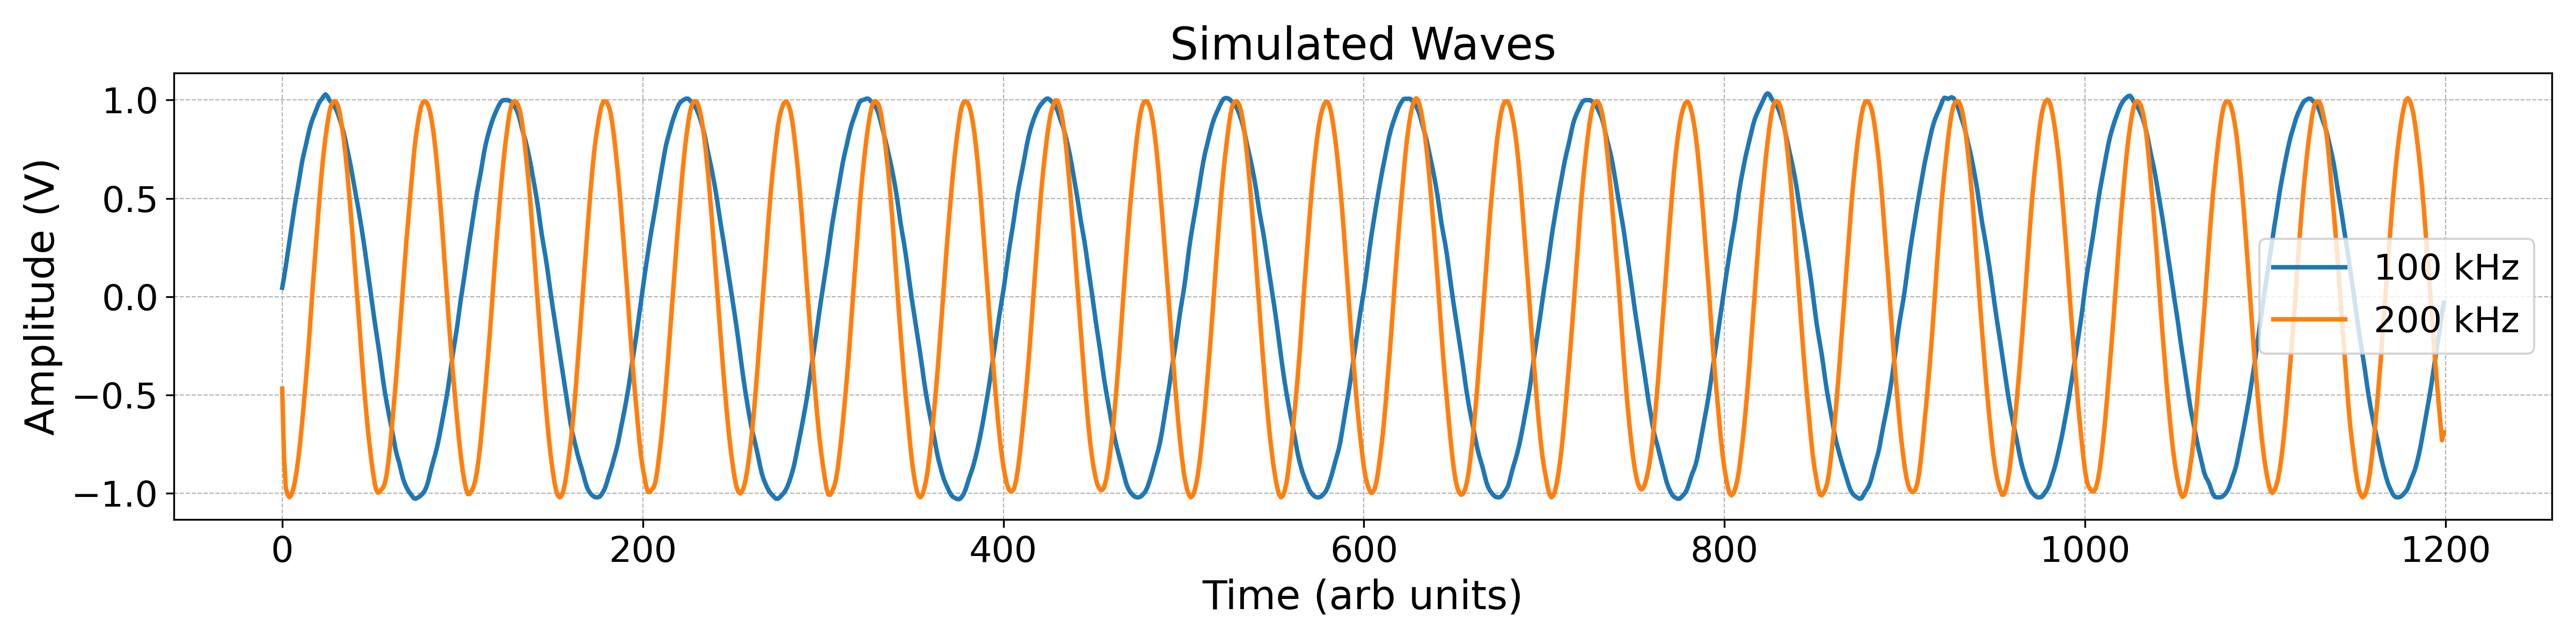
\includegraphics[width=\textwidth]{figs/waves-in.png}
    \caption{Sine waves created using the frequency generator to test the calculations implemented on the FPGA.}
    \label{fig:waves-in}
\end{figure}

In the subsequent parts we will treat the 100 kHz signal as the reference signal, $\lambda_R = 3000 m$ and the 200 kHz signal as the unknown signal. We expect to find $\lambda_X = 1500 m$.

\item \textbf{Calculating the wrapped phase:} 
We first calculate the phase of the signals generated as per the following equations,

\begin{equation}
\Phi_{\text{R}}(t) = \cos^{-1}(R)
\end{equation}

\begin{equation}
\Phi_{\text{X}}(t) = \cos^{-1}(X)
\end{equation}

Where $\Phi_{\text{R}}$ is the phase of the reference signal and $\text{R}$ is reference signal. Similarly, $\Phi_{\text{X}}$ is the phase of the unknown signal and $\text{X}$ is unknown signal. 

The wrapped phase of the signals as illustrated in figure \ref{fig:wrp-ph} is calculated by multiplying the phase by the sign the original signal. 

\begin{equation}
\Phi_{\text{wR}}(t) = \cos^{-1}(R) \cdot \text{sgn}(R))
\end{equation}

\begin{equation}
\Phi_{\text{wX}}(t) = \cos^{-1}(X) \cdot \text{sgn}(X)
\end{equation}

\begin{equation}
R = \cos (\Phi_{\text{R}(t)})
\end{equation}

\begin{equation}
X = \cos (\Phi_{\text{X}(t)})
\end{equation}

\begin{equation}
\Phi_{\text{X}}(t) = \cos^{-1}(X) \cdot \text{sgn}(X)
\end{equation}

Here, \( \text{sgn}(x) \) is the sign function, which returns -1 for \( x < 0 \), 0 for \( x = 0 \), and 1 for \( x > 0 \).

\begin{figure}[H]
    \centering
    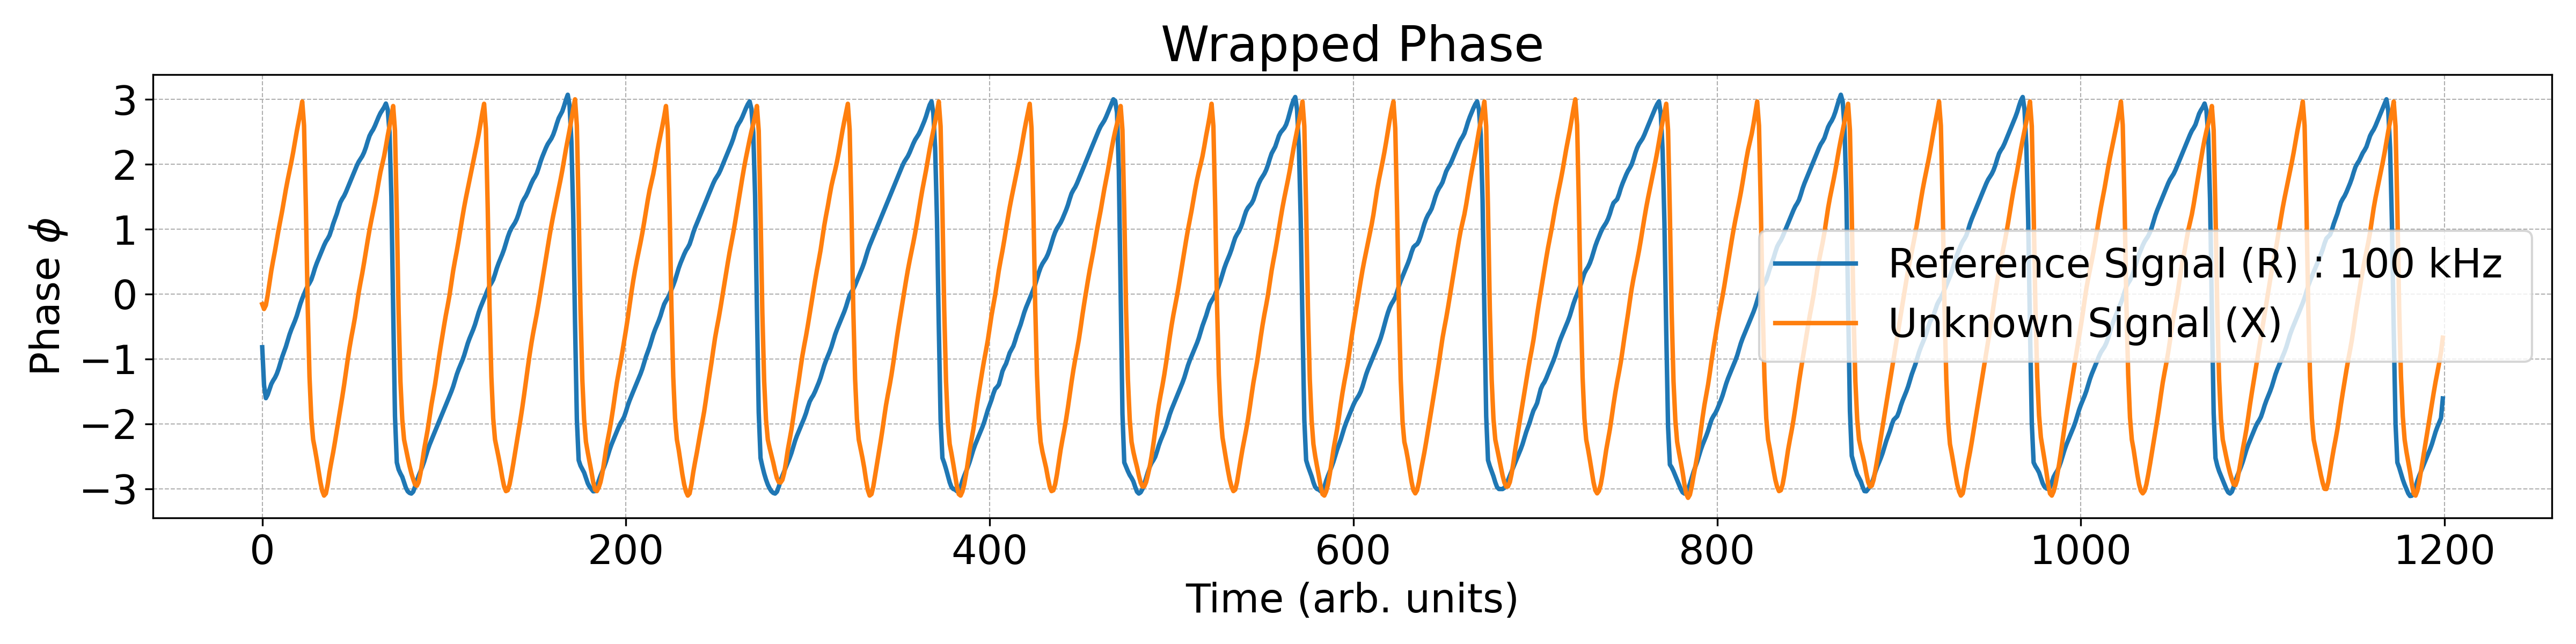
\includegraphics[width=\textwidth]{figs/wrp-ph.png}
    \caption{Wrapped phase of the input signals}
    \label{fig:wrp-ph}
\end{figure}

\item \textbf{Unwrapping the phase:} The unwrapped phase of the signals is calculated to avoid the abrupt jumps between $-\pi$ and $\pi$ that occur in the phase as computed by the $\cos^{-1}$ function. These jumps can be misleading when the phase is plotted, making the phase appear to change rapidly when it is actually changing slowly.

We calculate the unwrapped phase using an algorithm that adds or subtracts multiples of $2\pi$ to each phase angle to minimize the jump between consecutive angles.

The unwrapped phase of a signal can be represented as follows:

Let's denote the phase of the signal as $\phi(t)$. The unwrapped phase, $u(t)$, can be defined as follows:

\begin{enumerate}
    \item Set $u(t_0) = \phi(t_0)$ for the first time point $t_0$.
    \item For each subsequent time point $t_i$, compute the difference $\Delta \phi = \phi(t_i) - \phi(t_{i-1})$.
    \item If $\Delta \phi > \pi$, then $u(t_i) = u(t_{i-1}) + \Delta \phi - 2\pi$.
    \item If $\Delta \phi < -\pi$, then $u(t_i) = u(t_{i-1}) + \Delta \phi + 2\pi$.
    \item Otherwise, $u(t_i) = u(t_{i-1}) + \Delta \phi$.
\end{enumerate}

This algorithm ensures that the unwrapped phase $u(t)$ changes smoothly and avoids jumps greater than $\pi$. Figure \ref{fig:unwrp-ph} left, shows the unwrapped phase captured from the output of the FPGA.

\begin{figure}[H]
    \centering
    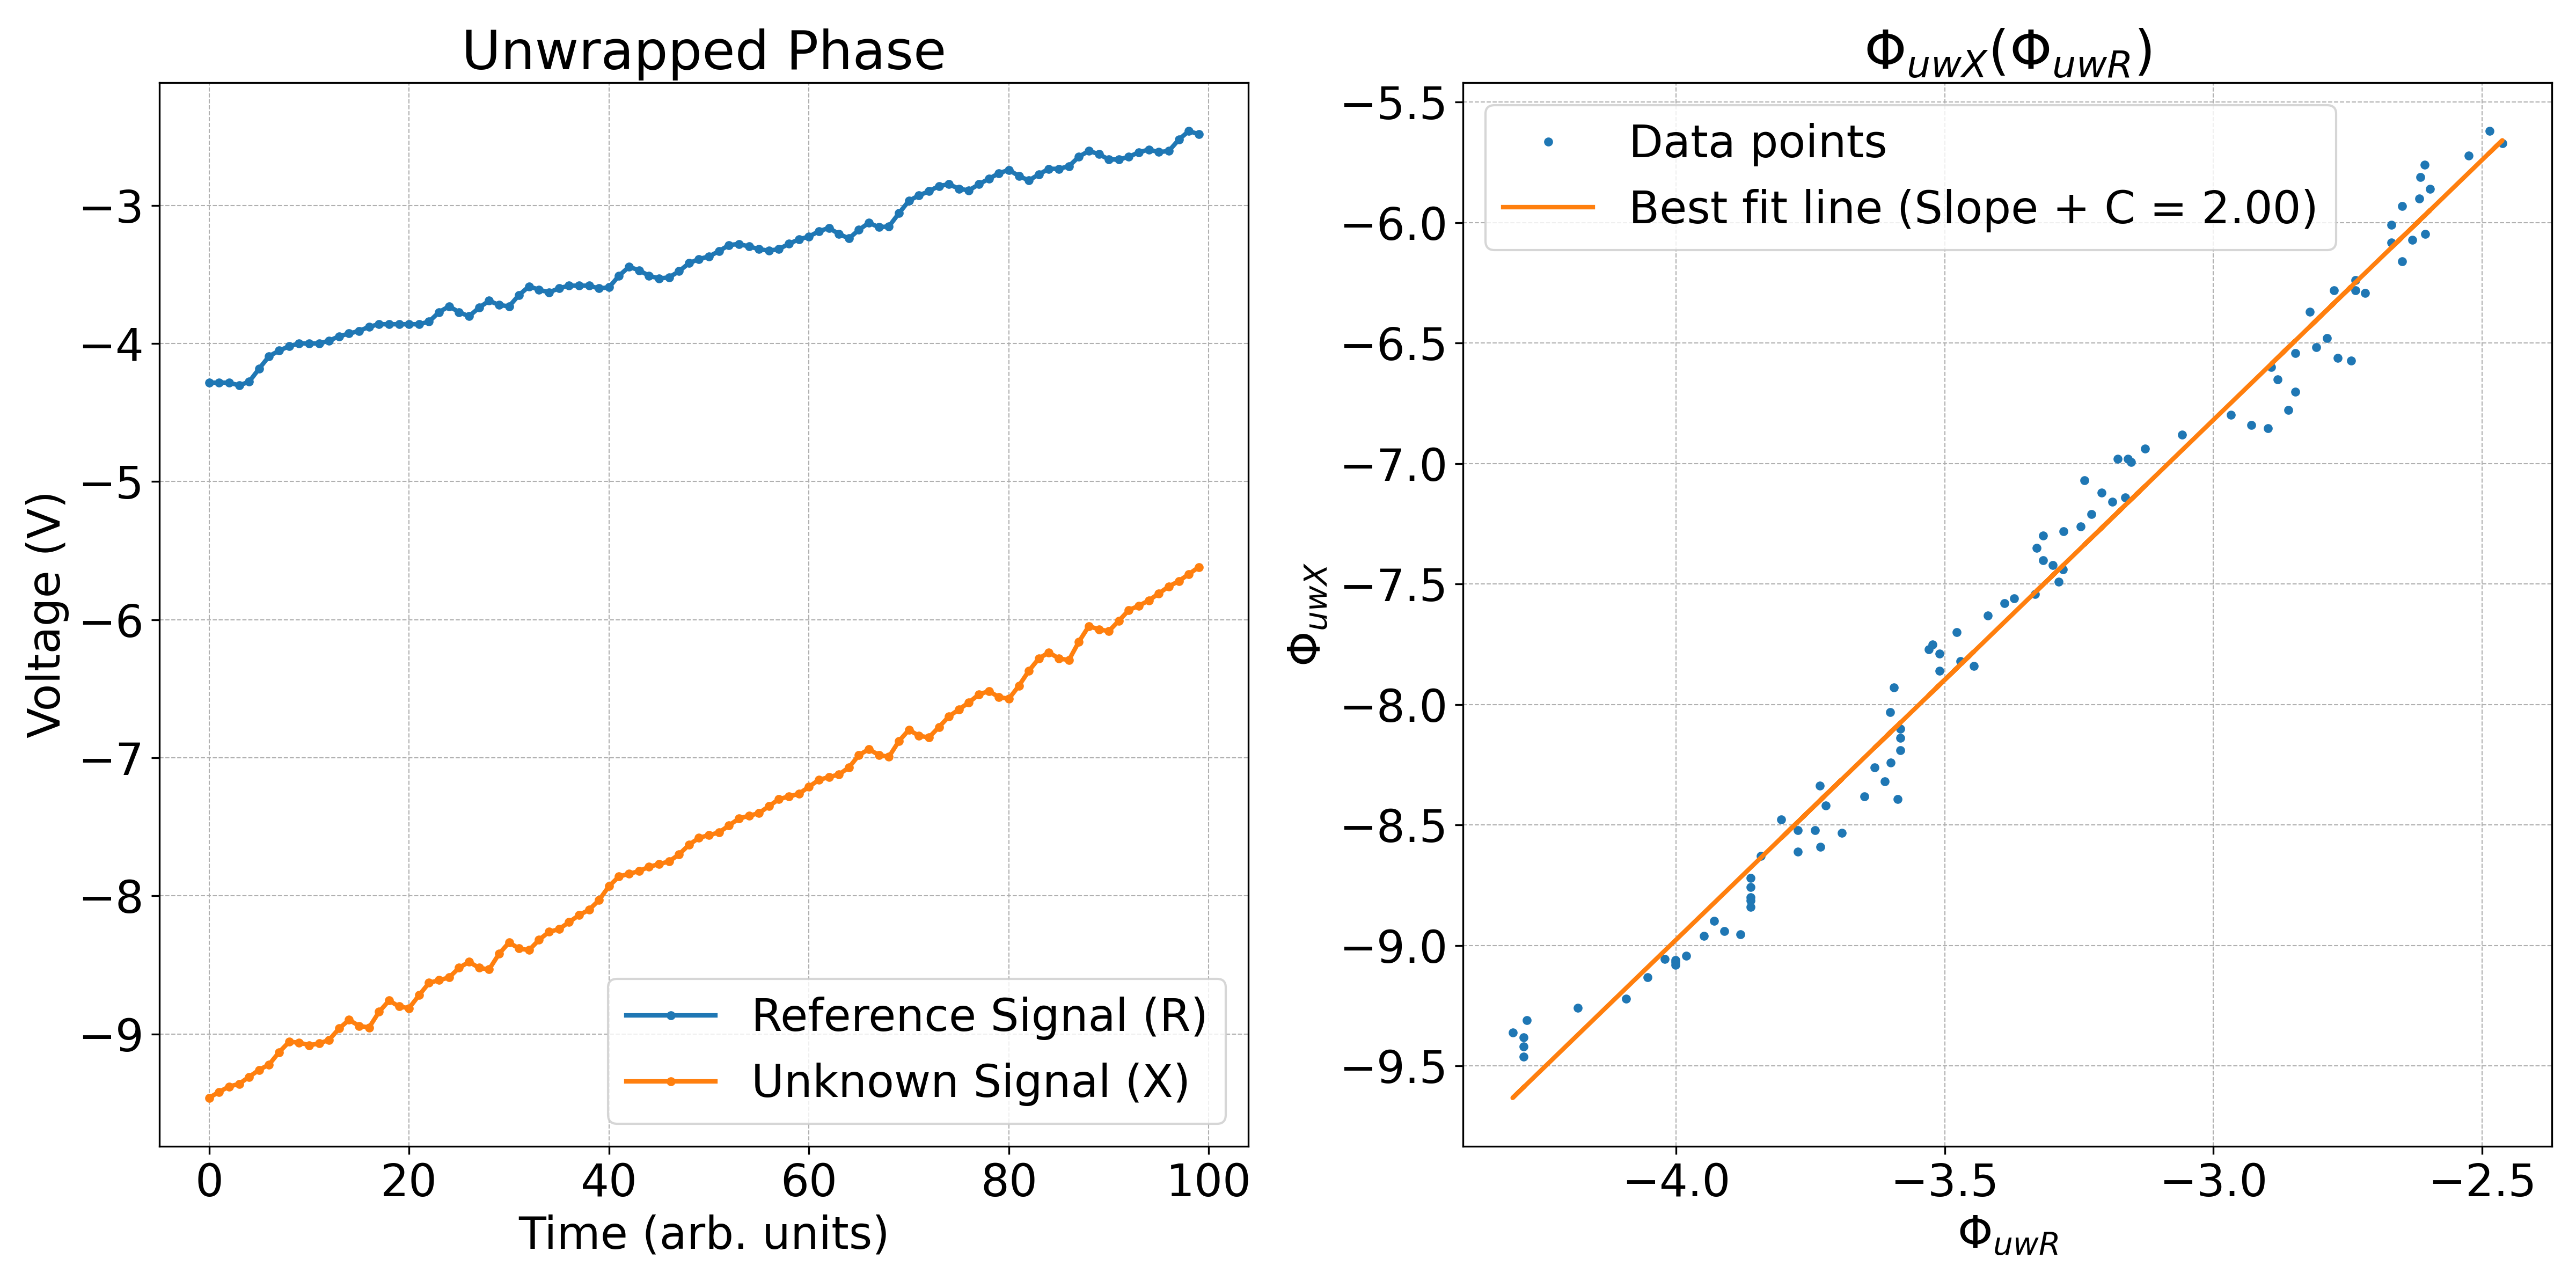
\includegraphics[width=\textwidth]{figs/unwrp-ph.png}
    \caption{\textbf{Left:} Unwrapped phases of the input signals phases $\Phi_{\text{uwX}}$, $\Phi_{\text{uwR}}$ \linebreak \textbf{Right:} Best fit line of $\Phi_{uwX}(\Phi_{uwR})$ }
    \label{fig:unwrp-ph}
\end{figure}

The phase shifts for each wavelength is linearly related to the displacement $\Delta(t)$ given by the s-curve. So, we can define the unwrapped phases as :

\begin{equation}
\Phi_{\text R} = k_R \cdot \Delta(t) + \Phi_{\text 0,R}
\label{eq-phR}
\end{equation}

\begin{equation}
\Phi_{\text X} = k_X \cdot \Delta(t) + \Phi_{\text 0,X}
\label{eq-phX}
\end{equation}

Here, $k_R$ and $k_X$ are the wave vectors for reference wavelength and the unknown wavelength respectively. We can determine the relation between the two phases, starting with equation \ref{eq-phR} where

\begin{equation}
\Delta(t) = \frac{\Phi_{\text R} - \Phi_{\text 0,R}}{k_R}
\end{equation}

substituting this into the equation \ref{eq-phX} gives:

\begin{equation}
\Phi_{\text X} = k_X \cdot \frac{\Phi_{\text R} - \Phi_{\text 0,R}}{k_R} + \Phi_{\text 0,X}
\end{equation}

Simplifying,

\begin{equation}
\Phi_{\text X} = \frac{k_X}{k_R} \cdot \Phi_{\text R} + C
\label{eq-phX-2}
\end{equation}

\item \textbf{Determining the unknown wavelength:} Finally, we determine the unknown wavelength $\lambda_X$. Using equation \ref{eq-phX-2} we can express the unknown wavelength $\lambda_X$ as

\begin{equation}
    \lambda_X = \frac{1}{m} \cdot \lambda_R 
    \label{wl-result}
\end{equation}

where, $m$ is the slope of the best-fit line \footnote{The part up until we get the unwrapped phase has been done on the FPGA, the linear regression has been done in python. It is in the process of being implemented on the FPGA.} of the function $\Phi_{uwX}(\Phi_{uwR})$ and $C$ is phase offset of the wrapped phase of the unknown signal which we saw in figure \ref{fig:wrp-ph}.

From equation \ref{wl-result} we calculate $\lambda_X$ for the signals being tested, 

\begin{equation}
    \lambda_X = \frac{1}{1.98} \cdot 3000m = 1515.15 m
\end{equation}

the expected result was $1500 m$, the result we get is off by approximately 8 \%. This issue is still being investigated, it could be due to the resolution of the oscilloscope used to capture the data or it could be a bug in the system verilog code. In theory this method works, so re-evaluating the system should help in rectifying this issue.

\end{enumerate}

\section{Corrections}\label{wavel-extraction}

In this section, we will discuss the Edlén Equation, a commonly used formula for calculating the refractive index of air. This equation, which accounts for various parameters such as temperature, pressure, and light wavelength, is a practical tool in fields like physics and engineering where precise light measurements are necessary.

\subsection{The Edlén Equation}

The \href{https://web.archive.org/web/20230608180923/https://emtoolbox.nist.gov/Wavelength/Documentation.asp}{Edlén Equation} is an empirical formula used to calculate the refractive index of air as a function of various parameters such as temperature, pressure, and wavelength of light \cite{Edln1953}. The equation is derived from experimental observations and is widely used in physics and engineering, particularly in the field of metrology, for high precision measurements of light \cite{Edln1966} \cite{Birch1993}.

\vspace{1em}
The equation is chosen for several reasons:

\begin{itemize}
\item \textbf{Precision:} The Edlén Equation provides a high degree of precision in calculating the refractive index of air, which is essential in many scientific and industrial applications.
\item \textbf{Applicability:} The equation takes into account various factors that can influence the refractive index of air, including temperature, atmospheric pressure, and humidity. This makes it versatile and applicable under different environmental conditions.
\item \textbf{Empirical validity:} The equation is based on empirical data and has been validated through numerous experiments and observations.
\end{itemize}

In its most basic form, the Edlén Equation can be represented as follows:

\begin{equation}
n - 1 = A + \frac{B}{\lambda^2} + \frac{C}{\lambda^4}
\end{equation}

where:

\begin{itemize}
\item $n$ is the refractive index of air,
\item $\lambda$ is the vacuum wavelength of light,
\item $A$, $B$, and $C$ are constants that depend on the temperature, pressure, and humidity of the air.
\end{itemize}

The constants $A$, $B$, and $C$ are determined empirically and can be adjusted to account for different atmospheric conditions and other factors. The constants $B$ and $C$ capture the dispersion of light, i.e., the dependence of the refractive index on the wavelength of light. The constant $A$ captures the pressure and temperature dependence of the refractive index.

\vspace{1em}
In practice, to calculate the refractive index of air using the Edlén Equation, one would need to know the vacuum wavelength of light, the temperature, pressure, and possibly the humidity and CO2 concentration. These values are plugged into the equation to compute the refractive index.

\vspace{1em}
We use the Edlén Equation to correct the possible errors in calculation of the unknown wavelength by multiplying the the unknown wavelength $\lambda_X$ by the refractive index given by the Edlén equation $n_E$

\begin{equation}
    \lambda_{\textbf{X}} = n_E \cdot \lambda_X
\end{equation}

\chapter{Discussion and Conclusion}

\section{Discussion}
The wave-meter presented in this report when completed would serve as quick way to measure wavelength of a the lasers frequently used in the experiments done within the group. With the current instrumentation as per figure \ref{exp-setup}, we estimate it be reliable in the 900 nm to 1700 nm range. These constraints arise from the dichroic mirror and the beam splitter that is being used, replacing these parts with alternatives with higher range should increase the range of wavelengths that are compatible with the wavemeter. The accuracy of the measurement is dependent on the precision of DACs of the FPGA and the accuracy of the wavelenght of the reference laser.

\vspace{1em}
It is also interesting to note that the cost of the equipment that is being used to build this wavemeter is a fraction of the the cost of commercially available devices. But, the complete comparison can be done after testing the completed wavemeter. 

\section{Conclusion}

In conclusion, this report has presented a comprehensive overview of the design and operation of an FPGA-based wavemeter. The wavemeter, is designed to determine unknown wavelengths by comparing them with a reference laser of known wavelength.

\vspace{1em}
The report has detailed the various stages involved in the operation of the wavemeter, from the setup of the optical components to the generation of control signals for the interferometer's translation stage, and the process of wavelength calculation. It has also discussed the application of the Edlén Equation as a means of correcting potential errors due to variations in the refractive index of air.

\vspace{1em}
Significant progress has been made in the development of the FPGA-based wavemeter, yet there remains a considerable amount of work to be done. The next stages of development will involve a combination of hardware refinement, software development, and rigorous testing. The principles and methodologies outlined in this report provide a solid foundation for these ongoing efforts. The ultimate goal is to develop a reliable, accurate, and versatile wavemeter. The forthcoming steps will involve rigorous testing and validation to ensure the wavemeter's performance and accuracy meet the desired standards.

\chapter{Outlook}



\section{Development of the wave-meter}

The development of the FPGA-based wavemeter is an ongoing project with several key areas identified for future work. The following sections outline the main areas of focus for the next stages of development.

\subsection{Linear Regression Algorithm}

The current implementation of the wavemeter relies on a linear regression algorithm to determine the slope of the best-fit line in the $\Phi_{\text X}$ vs $\Phi_{\text R}$ plot from figure \ref{fig:unwrp-ph}. This slope is crucial for calculating the unknown wavelength $\lambda_X$. Future work will focus on refining this algorithm to improve its accuracy and reliability. This could involve exploring different regression techniques, implementing error checking and correction mechanisms, and optimizing the algorithm for performance on the FPGA.

\subsection{Optical Setup}

The optical setup of the wavemeter, including the lasers, Michelson interferometer, and photodetectors, is another area of focus. Future work will involve fine-tuning this setup to ensure optimal performance. This could include adjusting the alignment of the optical components, experimenting with different types of lasers and photodetectors, and exploring ways to minimize noise. 

\vspace{1em}
We also have in mind an alternative design for the translation stage which can relax requirements of allotments by using cornered mirrors. Illustrated in the Appendix figure \ref{fig:cor-mirr-setup} Upgrades like these can be done after the development of all the required software is complete and the current setup is tested. 

\subsection{FPGA and Web-Interface Connections}

The connection between the FPGA and the web interface is a crucial component of the wavemeter system. Future work will focus on completing and testing these connections to ensure reliable data transmission and control. This could involve developing custom communication protocols, implementing error checking and correction mechanisms, and optimizing the system for performance and reliability.

\subsection{Testing and Validation}

Once the above components have been developed and refined, the next step will be to thoroughly test and validate the wavemeter. This will involve conducting a series of experiments to measure the wavelength of unknown signals and comparing the results with known values. The goal of this testing phase will be to assess the accuracy, precision, and reliability of the wavemeter, and to identify any areas that may need further refinement.


\bibliographystyle{ieeetr}  
\bibliography{sources}

\appendix
\chapter{Appendix}\label{apx:morestuff}

\begin{figure}[H]
    \centering
    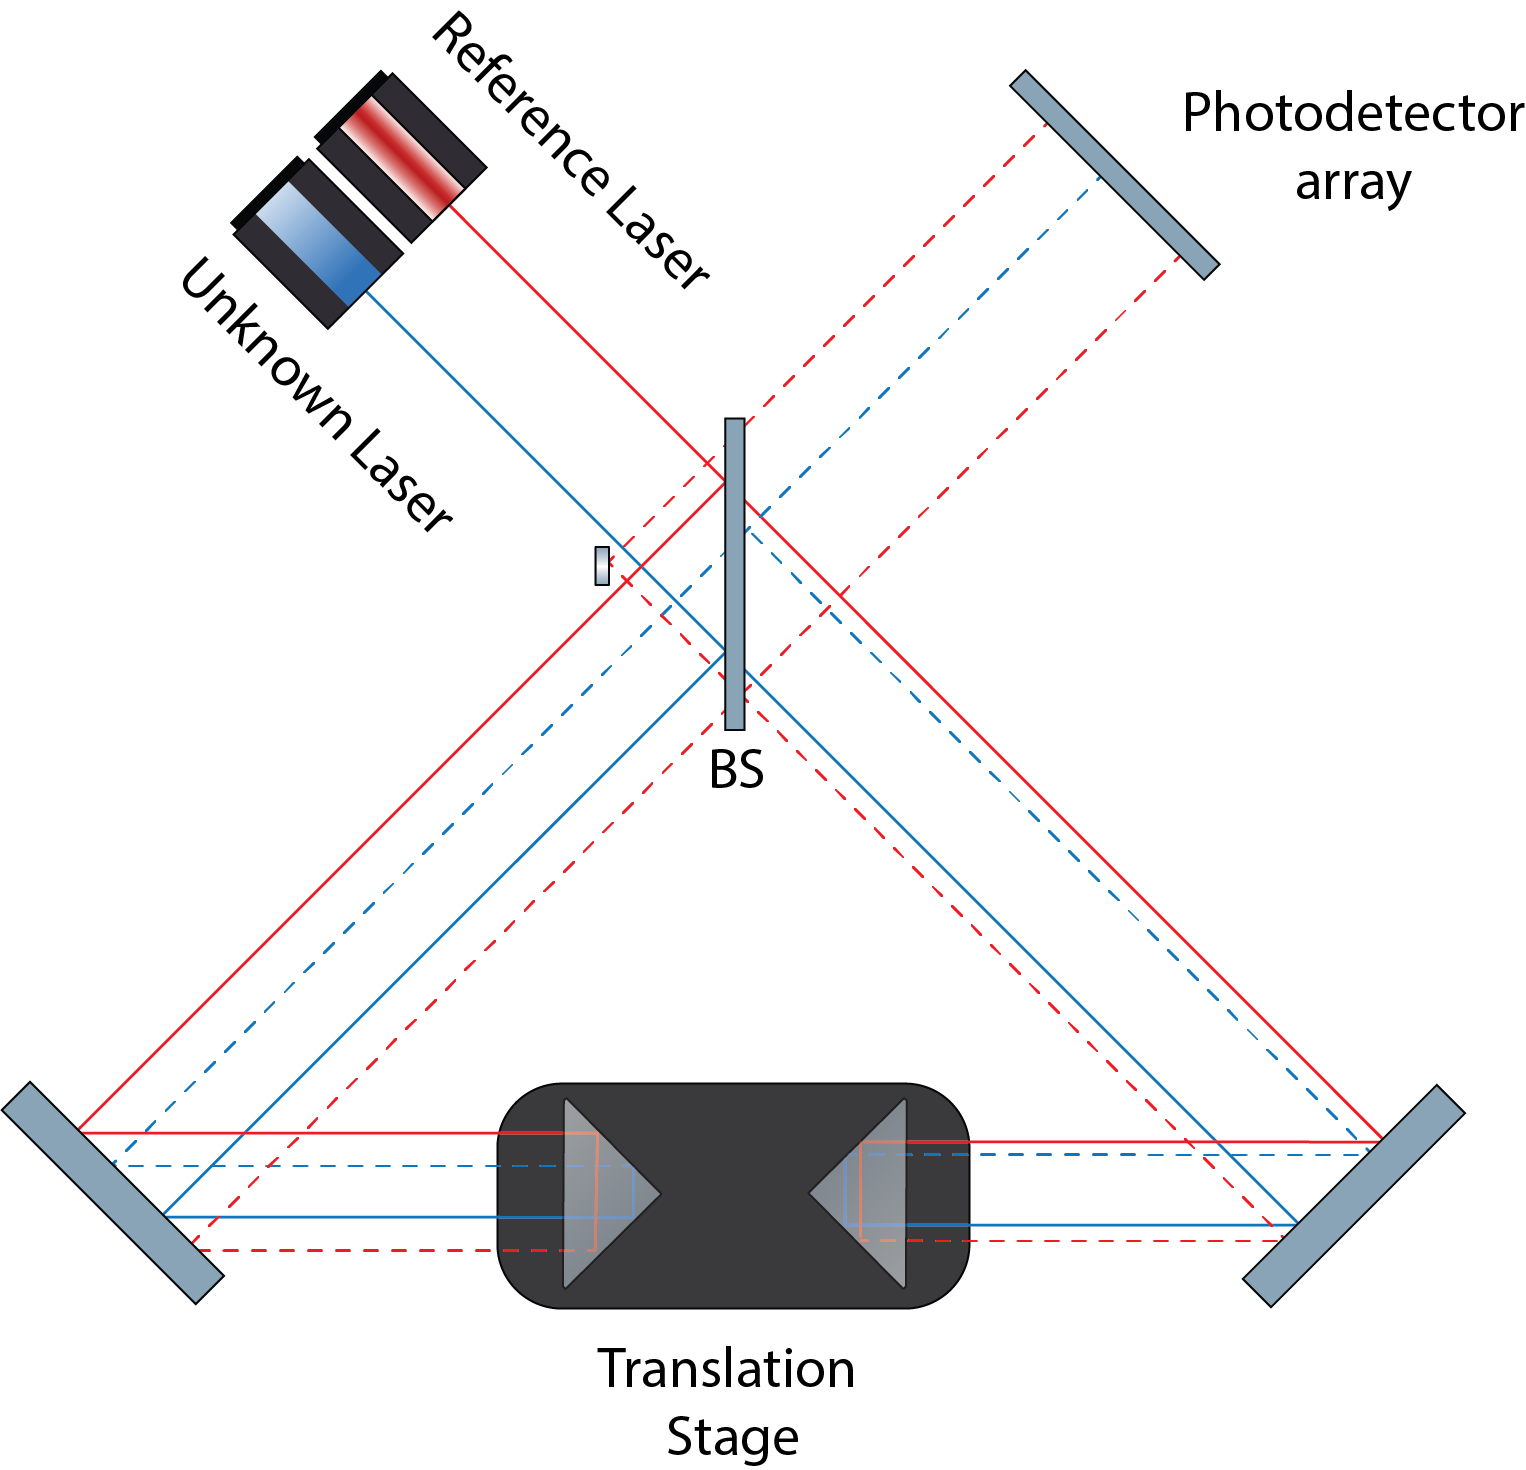
\includegraphics[width=0.5\textwidth]{figs/cor-setup.png}
    \caption{Alternative setup with corner mirrors.}
    \label{fig:cor-mirr-setup}
\end{figure}

\begin{equation}
    m = \frac{k_X}{k_R} = \frac{\lambda_R}{\lambda_X}
\end{equation}

\begin{equation}
    \lambda_X = \frac{\lambda_R}{m}
\end{equation}

\begin{equation}
y(t) = \frac{1}{6} \cdot j t^3
\end{equation}



\end{document}


